\documentclass{article}
\usepackage[utf8]{inputenc}
\usepackage{hyperref}
\usepackage{float}
\usepackage[table,xcdraw]{xcolor}
%\usepackage[sort&compress,square,comma,authoryear]{natbib}
\usepackage{booktabs}
\usepackage{graphicx}
\graphicspath{{Figures/}}
\usepackage{longtable}

\usepackage[
backend=biber,
style=authoryear,
sorting=nyt % sort by name year title
]{biblatex}
\addbibresource{Ref_invertebrate_DB.bib}

\title{ OUTLINE: Harmonized macroinvertebrate trait database, Aggregation of traits, Trait definitions, Sources }
\author{}%Stefan Kunz 
\date{}%June 2019


\begin{document}
%TODO: Use citep & citet instead of cite
\maketitle

\section{Introduction}

Intro: For what are traits used?\\
Knowledge on macroinvertebrate traits $\rightarrow$ trait databases
\\
\\
\\
Studies that use information on aquatic invertebrate traits from different regions
and/or aggregate trait information are increasing %! Change wording & State examples: Brown Paper
\\
\\
\\
%!Goal of our analysis:
In this paper we examine difficulties that ecologists face when using 
different macroinvertebrate trait databases together. We explore the 
effect of different decisions researches have to make when working with
trait data from several regions/sources, involving harmonization, 
handling different codings, normalization, and aggregation of traits.
\\
\\
\\
%! Trait terminology
%TODO: Apply unified terminology -> Use Schmera et al's suggestion?

One of the problems in macroinvertebrate trait research is the use
of inconsistent terminology across studies (but see \cite{schmera_proposed_2015}). 
For example, some studies used the term "trait" to describe a general 
organismal property like "generations per year" (\cite{statzner_reproductive_1997}, 
\cite{ussegliopolatera_biological_2000}), while in other studies this 
term was related to trait categories/states like "bi/multivoltine" 
(\cite{haybach_use_2004}, \cite{vieira_database_nodate}). 
Here, we follow the proposal of Schmera et al. (2015) and use the term 
\textit{trait} for a morphological, physiological, or phenological 
feature measurable at the individual organism (e.g. tegument, gills, etc.) 
and the term \textit{grouping feature} to describe a general property 
of related organismal traits (e.g. respiration).
\\
\\
\\
%!What we did:
Therefore, we harmonized six grouping features from four trait databases and 
aggregated the trait information to family level. % ?Name Traits
We discuss the harmonization and show the effect of different ways of aggregating 
traits (inter alia Problem of different coding styles (fuzzy vs binary)).
We also present an overview of differences in trait definitions among databases.
Finally, our paper compares the references for the trait information that 
were specified in the trait databases we used.




\section{Description of harmonized trait database} %TODO: Change heading to be more expressive

% TODO Give a motivation (better in introduction?)
The harmonized database consists of the available information on aquatic 
insect traits for the regions Europe, North America, Australia, and New Zealand
and comprises the grouping features locomotion, feeding mode, respiration, 
voltinism, size, and body form. The pattern of development (holometabolous or hemimetabolous) 
was added as an additional grouping feature based on the orders of the taxa 
included in each database. 
% TODO: Few words why these traits have been selected
% TODO: Reasoning why no ecological traits have been used
Trait information for Australia and New Zealand were retrieved from 
single database. For Europe we gathered trait information from the 
freshwaterecology trait database (\url{https://www.freshwaterecology.info/}) 
and complemented missing information with the 
Tachet trait database (\cite{usseglio-polatera_biomonitoring_2000}). 
North American macroinvertebrate traits were retrievied from Laura Twardochleb and 
complemented by trait information from Vieira et al (\cite{vieira_database_nodate}). 
% TODO Mention restriction to certain orders
We did not use the entire data on macroinvertebrates, 
but limited our analysis to orders of aquatic insects that occurred in all used
databases, specifically the orders:
...
% TODO: Insert citation
Table \ref{tab:trait_databases} gives an overview of the used databases. \\ 
In the following paragraphs, we describe the data processing steps required to 
establish a harmonized macroinvertebrate trait database. 

\begin{table}[H]
    \centering
    \caption{Overview of trait databases.}
    \label{tab:trait_databases}
    \begin{tabular}{lll}
    \toprule
   Region & Coding of trait states & Reference \\ 
    \hline
   Europe & Largely fuzzy & \cite{schmidt-kloiber_www.freshwaterecology.info_2015}\\ 
   Central Europe & Fuzzy coded & \cite{usseglio-polatera_biomonitoring_2000} \\ 
   North America & Largely binary & \cite{vieira_database_nodate}\\
   North America & Largely binary & cite Laura Twardochleb \\
   Australia & Binary \& fuzzy coding  & \cite{kefford_ben_AST_DB_2019}\\ 
   New Zealand & Fuzzy coded & \\ %TODO: Create entry for more recent NZ reference
    \bottomrule
    \end{tabular}
\end{table}

\begin{itemize}
    \item Various preprocessing steps: Taxonomical corrections; Range normalization [0-1] (e.g. in Australia); a few 
    words about spreadsheets etc?
    \item Harmonization 
    \item (RowSum) Normalization/Standardization %!Wording
    \item Aggregation of traits
\end{itemize}




\subsection{Harmonization of traits}
\begin{itemize}
    \item Harmonization process: See also Schmera 2015 et al 
    \item Differences in trait definitions
    \item Sources of traits
\end{itemize}

% !What is harmonization? & Why is it needed?
Harmonization of traits is the process of amalgamating several similar trait states
into a single trait state. Harmonization has to be undertaken when e.g. traits from
different sources (e.g. different regions) are compared and the traits have not
the same trait states. %?Give an example -> Clusteranalysis
\\
\\
\\
% !How was the harmonization done? -> technical aspect.
Traits that differed in their trait states among databases have been harmonised by 
condensing the trait states for each trait in such a way that in the end the same 
traits in all four databases consisted of the same trait states. 
This meant reducing the trait states to the smallest number of trait states that
occur for a particular trait among all databases. Thereby, trait states were 
amalgamated based on ecological knowledge or expert judgment. %!Wording 
Our approach of harmonizing the traits of the used databases is outlined in figures 
\ref{fig:harmon_overview_1} and \ref{fig:harmon_overview_2}. 

\begin{figure}[H]
   \centering
   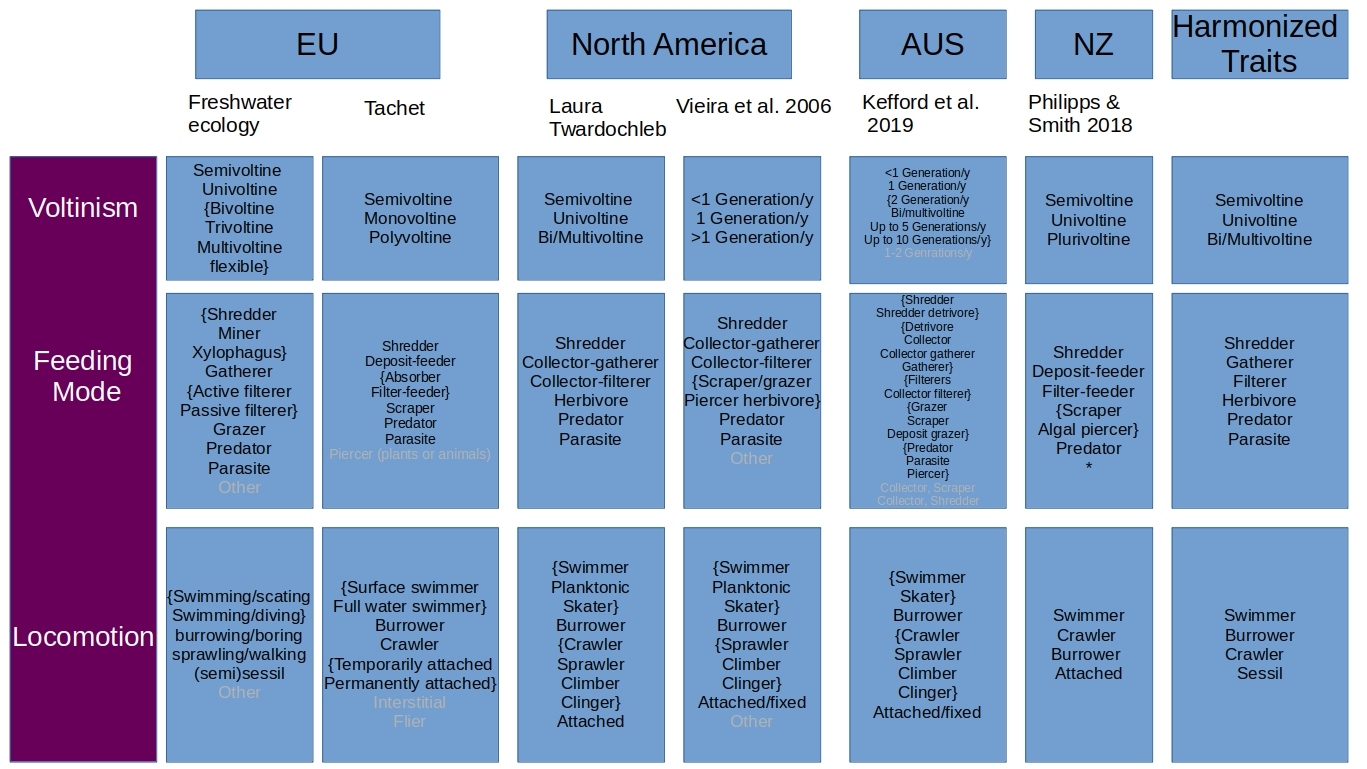
\includegraphics[width=16.5cm, height=10cm]{trait_overview1.jpg}
   \caption{Proposed harmonization scheme for the grouping features
   voltinism, feeding mode and locomotion. Shown are all traits for the 
   used grouping features in the investigated trait databases and 
   the harmonized traits in the end. Traits in curly brackets were 
   harmonized to one trait. Traits highlighted in Grey were omitted. \newline
   \textit{* Trait parasite was not available in New Zealand trait database.}
   }
   \label{fig:harmon_overview_1}
\end{figure}

\begin{figure}[H]
    \centering
    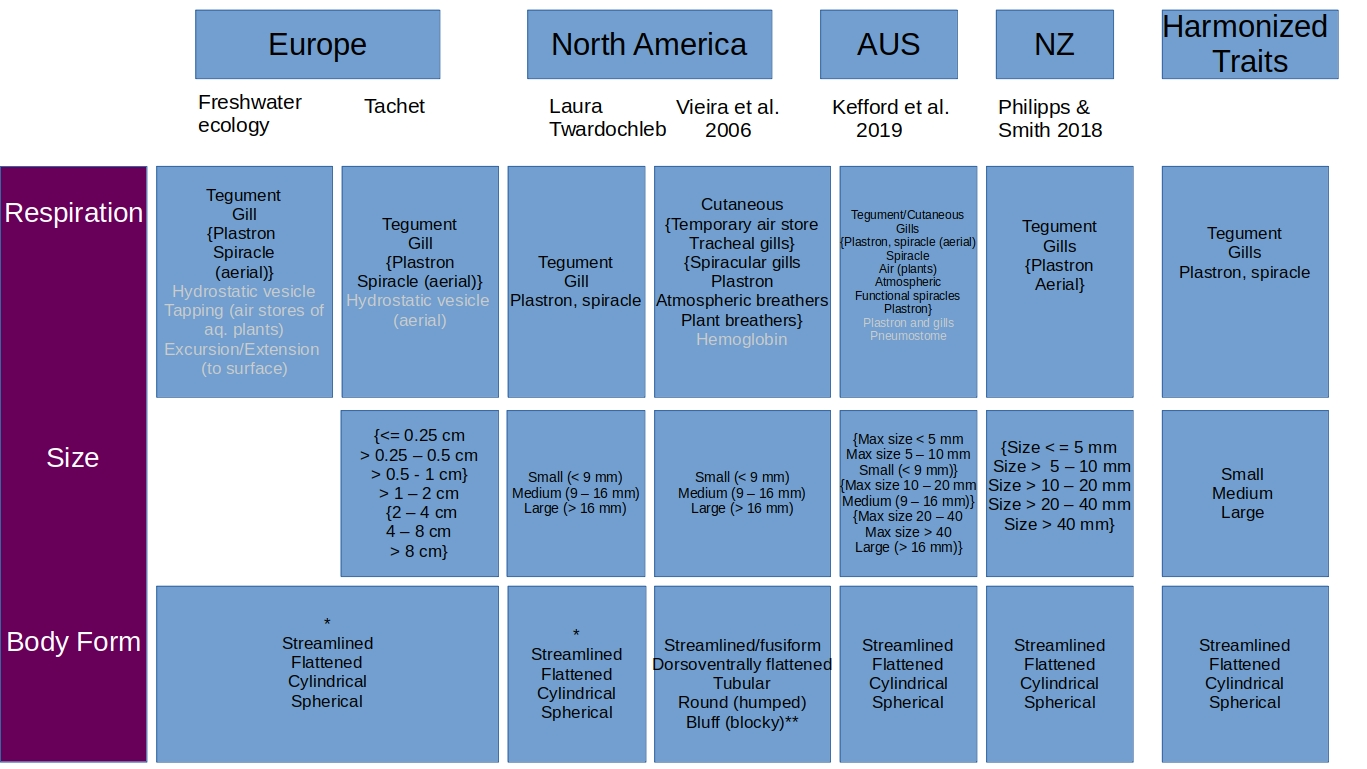
\includegraphics[width=16.5cm, height=10cm]{trait_overview2.jpg}
    \caption{Proposed harmonization scheme for the grouping features
    respiration, size and body form.\newline
    \textit{* Body form information provided by Philippe 
    Usseglio-Polatera.}\newline
    \textit{** Bluff(blocky) taxa have been reclassified
    by Philippe Usseglio-Polatera using the traits streamlined,
    flattened, cylindrical and spherical.} }
    \label{fig:harmon_overview_2}
 \end{figure}
 

\section{Aggregation of traits}

\begin{itemize}
    \item Describing \& testing different approaches
    \item Problem of coding of traits
\end{itemize}

\section*{Additional ideas}

Section Description of databases:
\begin{itemize}
    \item Describe different databases briefly?
    \item State goal of analysis $\rightarrow$ reference to second paper?
\end{itemize}

\end{document}